\subsubsection*{Le matin :}
La matiné a été passée a finaliser le travail d'hier.
J'ai aussi developé un package afin d'encapsuler la librairie Keras et donc de simplifier son utilisation.
Voici la forme du réseau :
\begin{figure}[H]
    \center
    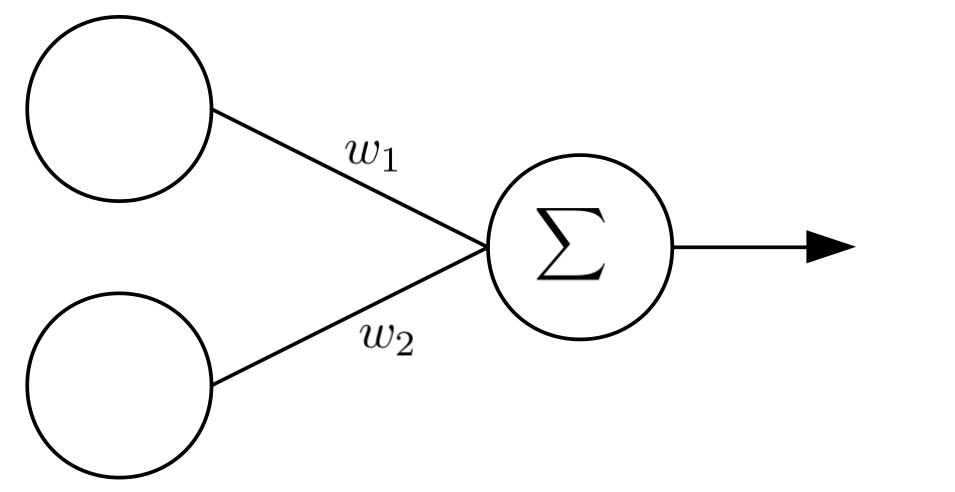
\includegraphics[height=\petit]{sources/pictures/network1.png}
	\caption{Réseau de neurone très simple}
	\label{n1}
\end{figure}
Le reseau vas essayer de faire varier les poids $w_1$ et $w_2$ afin de coller avec le fonction qui doit etre aprise.


\subsubsection*{L'après midi :}
On peut maintenant simplement faire apprendre au réseau une fonction simple.
Par exemple la moyenne :

\begin{figure}[H]
    \center
    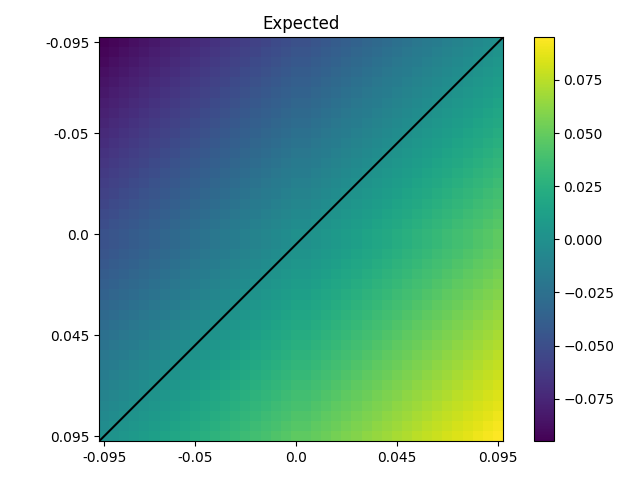
\includegraphics[height=\petit]{sources/data/moy/expected}
    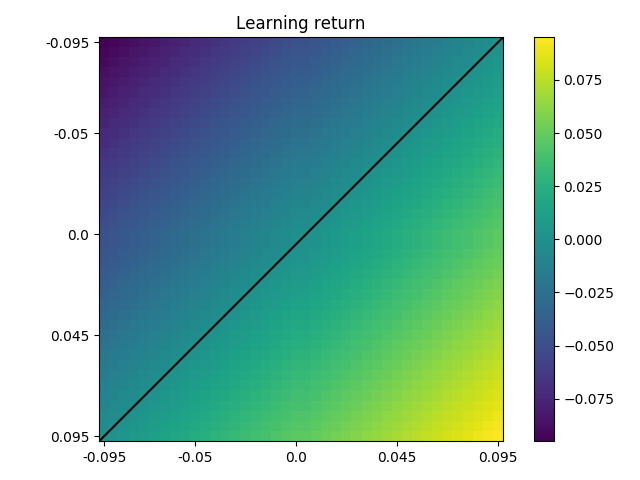
\includegraphics[height=\petit]{sources/data/moy/result}
	\caption{Apprentissage de la moyenne}
	\label{moy}
\end{figure}

Le graphique de droite est celui attendu et celui de gauche celui obtenu.
On peut voir que la descente de gradients se fait a merveille.
Aucunes difference ne sont visibles : en effet les poids associés aux deux noeuds sont les suivants :
\begin{equation*}
    w_1 = 0.50000010
    \;\;\;\;\;\;\;\;\;
    w_2 = 0.50000024
\end{equation*}
On peut voir qu'aux aproximations processeur, les poids sont les bons pour faire la moyenne de deux nombres :
\begin{equation*}
    m =\frac{n_1 + n_2}{2} = 0.5 \times n_1 + 0.5 \times n_2
\end{equation*}

